\chapter{Conclusions}
\label{chapter:conclusions}

This thesis has examined different technical solutions to managing, sharing and
publishing research data, focusing on sharing and publishing. The Table
\ref{table:solutions} shows the features of solutions presented and shows
how they differ in the context of research data publishing, whereas Table
\ref{table:management} shows the same solutions but in the context of research
data management during a research project. The Table
\ref{table:legend_colors} shows the legend that is used in Tables
\ref{table:solutions} and \ref{table:management}. Later in this section the
proposed requirements for a succescull research data management solution
are presented.

\label{table:legend_colors}
\captionof{table}{The color coding of the summary Tables \ref{table:solutions} and \ref{table:management}}
    \begin{tabularx}{\textwidth}{| >{\raggedright}p{3cm} | X |}
    \hline
    \textbf{Color and Mark} & \textbf{Meaning} \\
    \hline
    \multicolumn{1}{|c|}{\cellcolor{green}++} & The feature is well implemented and could be considered a strong point
                          in the solution \\
    \hline
    \multicolumn{1}{|c|}{\cellcolor{yellow}+} & The feature is implemented in the solutions in some way - it might need
                          some work to get up and running or the other features of the system can be used to
                          approximate the functionality \\
    \hline
    \multicolumn{1}{|c|}{\cellcolor{red}-}    & The feature is missing from the solution or can be found from the system but according
                          to user feedback is too hard to use and is a clear weak point of the system \\
    \hline
\end{tabularx}

In Tables \ref{table:solutions} and \ref{table:management} the IDA, Etsin, Avaa and PAS are a part of the
Finnish Open Science Initiative. Dataverse, Hydra, Zenodo, iRODS and CKAN are
open source solutions. EUDAT refers to the B2-offering\footnote{\url{http://eudat.eu/}},
of which the B2Share and B2Drop are considered to be a part of a reserch
data management and publication process. ACRIS is the Elsevier Pure instance
that is being trialed at Aalto University. GitHub is included in the
comparasion since it is a widely adopted tool for publishing and collaborating
on software projects.

The features used in the columns in Table \ref{table:solutions} are explained
below in Table \ref{table:solution_features}:


\label{table:solution_features}
\captionof{table}{The features being compared on Table \ref{table:solutions}}
    \begin{tabularx}{\textwidth}{| >{\raggedright}p{3cm} | X |}
    \hline
    \textbf{Feature} & \textbf{Explanation} \\
    \hline
    Data Storage    & Data storage means that the solution offers the chance to
                      save the actual research data to the system and not just links
                      to the datasets, for example\\
    \hline
    Metadata Storage &  Metadata storage means that the system has a structured way
                        of storing metadata anout datasets - this does not mean that
                        the system should contain actual research data, since some services
                        are built just as places to store metadata and point to datasets\\
    \hline
    Open Access Data    & System that implements this feature allows the datasets to be searched
                          and downloaded by the general public without restrictions to the use
                          of the datasets\\
    \hline
    Restricted Data    & Whereas open access data is available for all the world to see, systems
                         that implement the restriced data feature allow for a more fine grained
                         user management allowing datasets to be shared for restricted groups
                         of users\\
    \hline
    Long Term Archival    & Long term archival is archival for datasets that lasts for tens of years -
                            a lot longer than commodity hard drives last in active use (commodity
                            hard drives usually last from three to five years in active use)\\
    \hline
    Full Text Search    & Full text search refers to the ability to search the all the metadata
                          available in the system to find relevant datasets\\
    \hline
    Dataset Versionig    & Dataset versioning means that the system allows for uploading newer versions
                           of the already uploaded datasets without deleting the old datasets, since
                           someone might use and refer to the old datasets\\
    \hline
    Identifier Scheme    & Identifier scheme tells which, if any, persistent identifier schemese the
                           solution implements\\
    \hline
\end{tabularx}

From the solutions presented in Table \ref{table:solutions} the systems that
are designed primarily for research data publishing (Avaa, Dataverse, Hydra,
Zenodo, and CKAN) have almost all the features specified here. What some of
them are lacking is the ability to restrict access to the research data, which
is a requirement for some datasets that contain data that has some
confidentiality clauses. Avaa, for example, is a platform for nothing else than
completely open data making it an awkward choise for a university, for example.
None of these solutions implement long term archival,
which is an important feature going forward and a goal for future development.
These solutions are also remakrably similar, so any one of them could be used
to set up a research data publishing platform for a research institution.

The only solution for long term archival is PAS, which is in test phase as of
writing of this thesis. It ticks many boxes of the features, but it has to be
taken into accoung that the PAS system is only for long term archival and
can not be used for the normal publishing activity of research institutions.
It is also unclear at the moment how datasets for long term archival are
chosen, what kind of metadata long term archival requires and how the system
should integrate to existing and upcoming research data repositories.

The tools that have a lot of other functionality in addition to research data
publishing implement the features to a varying degree. iRODS, which is a tool
for managing data, is clearly not designed to be sharing platform for
research data. ACRIS has many other tasks as well, such as maintaining a the
publication profile of researchers and reporting publications. EUDAT's B2Share
offering offers a serviceable research data publication platform, but lacks the
ability to restrict access to the datasets. IDA is an iRODS based system, but
has some features for publishing datasets from the system. Biggest problem with
it is that it's perceived very hard to use by users.

Etsin is a metadata publication platform - it only contains metadata and links
to the actual location of the datasets. While this is valuable, separating the
research data from the metadata requires either integration between the storage
and metadata systems or more work from the users.

The identifier scheme is also a point of interest. Citing datasets is something
that has not been widely adopted, which means that in order to help that
adoption a well known identifier scheme should be used. It is good that there
is a Finnish identifier scheme, but if datasets want international recognition
an internationally known identifier scheme should be used.

The technical solutions with a focus on research data publishing fill their
role adequately. The user tests show that there are user experience and
uasbility improvements that could be done - those are detailed in Section
\ref{sec:prototype_outcomes}. What the user tests also show is that training
related to the options when it comes to research data publishing is lacking
and if the culture and willingness to share research data would be improved
that would include a concious effort from the university side.

\begin{sidewaystable}
    \caption{Existing solutions in light of research data publishing}
    \label{table:solutions}
    \resizebox{\textwidth}{!}{
        \renewcommand{\arraystretch}{2.0}
        \begin{tabular}{| l | c | c | c | c | c | c | c | c | c |}
            \cline{3-10}\cline{1-1}
            \rowcolor{top-level-blue}
            \vspace{1 mm}
            \textbf{Tool} &\cellcolor{white}& \textbf{Data Storage} & \textbf{Metadata Storage} & \textbf{Open Access Data} & \textbf{Restricted Data} & \textbf{Long Term Archival} & \textbf{Full Text Search} & \textbf{Dataset Versioning} & \textbf{Identifier Scheme} \\
            \cline{3-10}\cline{1-1}
            \cellcolor{first-column-blue}IDA     && \cellcolor{green}++ & \cellcolor{green}++ & \cellcolor{yellow}+  & \cellcolor{yellow}+  & \cellcolor{red}-  &  \cellcolor{green}++ & \cellcolor{red}-  & \cellcolor{green}URN \\
            \cline{3-10}\cline{1-1}
            \cellcolor{first-column-blue}Etsin   && \cellcolor{red}-  & \cellcolor{green}++ & \cellcolor{red}-  & \cellcolor{red}-  & \cellcolor{red}-  &  \cellcolor{green}++ & \cellcolor{red}-  & \cellcolor{green}URN \\
            \cline{3-10}\cline{1-1}
            \cellcolor{first-column-blue}Avaa    && \cellcolor{green}++ & \cellcolor{green}++ & \cellcolor{green}++ & \cellcolor{red}-  & \cellcolor{red}-  &  \cellcolor{green}++ & \cellcolor{red}-  & \cellcolor{green}URN \\
            \cline{3-10}\cline{1-1}
            \cellcolor{first-column-blue}Dataverse && \cellcolor{green}++ & \cellcolor{green}++ & \cellcolor{green}++  & \cellcolor{green}++ & \cellcolor{red}-  &  \cellcolor{green}++ & \cellcolor{yellow}+  & \cellcolor{green}DOI/Handle \\
            \cline{3-10}\cline{1-1}
            \cellcolor{first-column-blue}Hydra    && \cellcolor{green}++ & \cellcolor{green}++ & \cellcolor{green}++ & \cellcolor{green}++ & \cellcolor{red}-  &  \cellcolor{green}++ & \cellcolor{yellow}+  & \cellcolor{green}DOI \\
            \cline{3-10}\cline{1-1}
            \cellcolor{first-column-blue}Zenodo   && \cellcolor{green}++ & \cellcolor{green}++ & \cellcolor{green}++ & \cellcolor{yellow}+  & \cellcolor{red}-  &  \cellcolor{green}++ & \cellcolor{yellow}+  & \cellcolor{green}DOI \\
            \cline{3-10}\cline{1-1}
            \cellcolor{first-column-blue}EUDAT    && \cellcolor{green}++ & \cellcolor{green}++ & \cellcolor{green}++ & \cellcolor{yellow}+  & \cellcolor{red}-  &  \cellcolor{green}++ & \cellcolor{yellow}+  & \cellcolor{green}Handle \\
            \cline{3-10}\cline{1-1}
            \cellcolor{first-column-blue}iRODS    && \cellcolor{green}++ & \cellcolor{green}++ & \cellcolor{red}-  & \cellcolor{red}-  & \cellcolor{red}-  &  \cellcolor{green}++ & \cellcolor{yellow}+  & \cellcolor{red}- \\
            \cline{3-10}\cline{1-1}
            \cellcolor{first-column-blue}CKAN     && \cellcolor{green}++ & \cellcolor{green}++ & \cellcolor{green}++ & \cellcolor{green}++ & \cellcolor{red}-  &  \cellcolor{green}++ & \cellcolor{yellow}+  & \cellcolor{yellow}+ \\
            \cline{3-10}\cline{1-1}
            \cellcolor{first-column-blue}ACRIS    && \cellcolor{red}-  & \cellcolor{yellow}+  & \cellcolor{yellow}+  & \cellcolor{yellow}+  & \cellcolor{red}-  &  \cellcolor{green}++ & \cellcolor{red}-  & \cellcolor{yellow}+ \\
            \cline{3-10}\cline{1-1}
            \cellcolor{first-column-blue}PAS      && \cellcolor{green}++ & \cellcolor{green}++ & \cellcolor{green}++ & \cellcolor{red}-  & \cellcolor{green}++ &  \cellcolor{green}++ & \cellcolor{red}-  & \cellcolor{green}URN \\
            \cline{3-10}\cline{1-1}
            \cellcolor{first-column-blue}GitHub   && \cellcolor{green}++ & \cellcolor{yellow}+  & \cellcolor{green}++ & \cellcolor{green}++ & \cellcolor{red}-  &  \cellcolor{green}++ & \cellcolor{green}++ & \cellcolor{green}DOI \\
            \cline{3-10}\cline{1-1}
        \end{tabular}
    }
\end{sidewaystable}

\iffalse
\begin{sidewaysfigure}
    \begin{centering}
        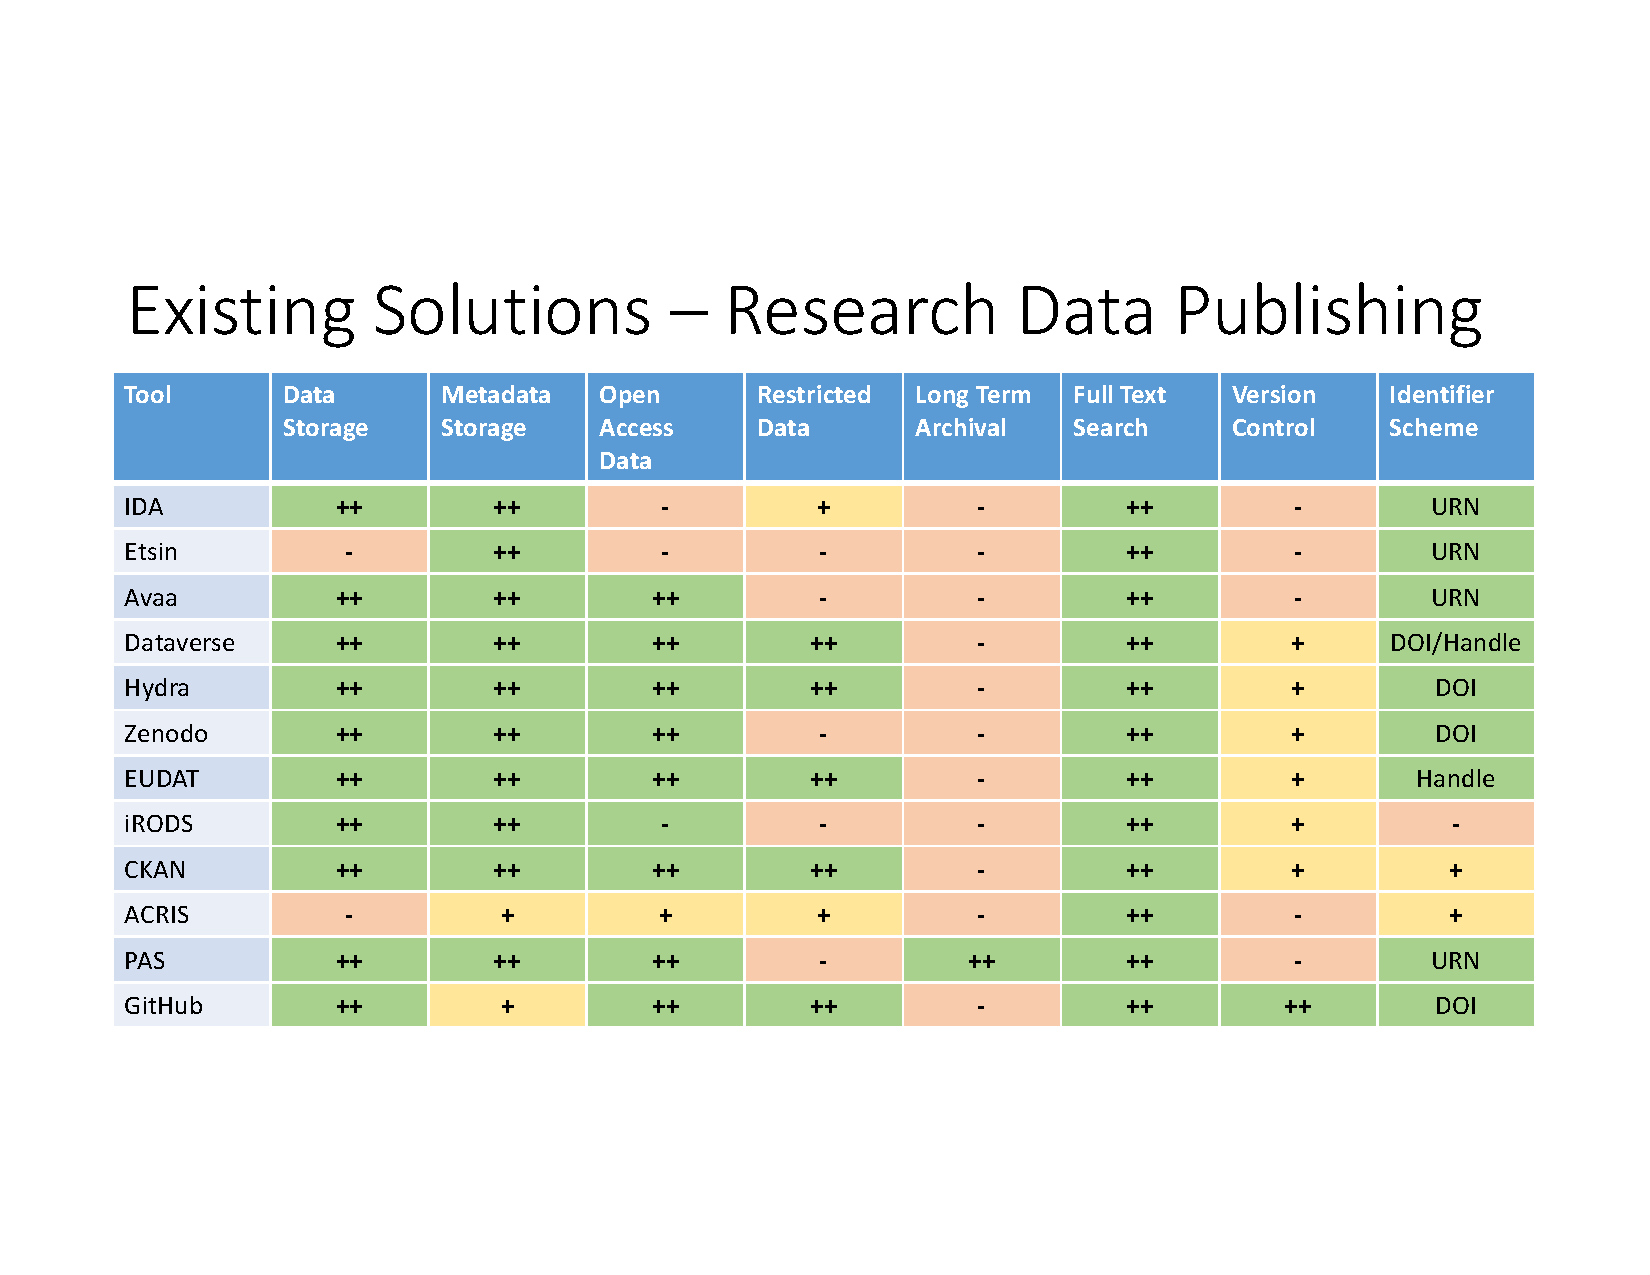
\includegraphics[width=\textwidth]{images/publishing}
    \end{centering}
    \caption{A placeholder for the latex table}
    \label{fig:solutions}
\end{sidewaysfigure}
\fi

Research data publishing is the end goal of research data management, and
Table \ref{table:management} shows the same tools compared previously in
the contex of research data publishing tbeing compared in the light
of research data management during the research process.

\begin{sidewaystable}
    \caption{Existing solutions in light of research data management}
    \label{table:management}
    \resizebox{\textwidth}{!}{
        \renewcommand{\arraystretch}{2.0}
        \begin{tabular}{| l | c |c | c | c | c | c | c | c | c |}
            \cline{3-10}\cline{1-1}
            \rowcolor{top-level-blue}
            \vspace{1 mm}
            \textbf{Tool} &\cellcolor{white}& \textbf{\vtop{\hbox{\strut File Sharing}\hbox{\strut With Partners}}} & \textbf{\vtop{\hbox{\strut File Editing}\hbox{\strut  With Partners}}} & \textbf{Workflow Sharing} & \textbf{Comments On Files} & \textbf{Web Interface} & \textbf{\vtop{\hbox{\strut Command Line}\hbox{\strut Interface}}} & \textbf{Desktop Interface} & \textbf{\vtop{\hbox{\strut Integrated}\hbox{\strut Data Collection}}} \\
            \cline{3-10}\cline{1-1}
            \cellcolor{first-column-blue}IDA         && \cellcolor{green}++ & \cellcolor{green}++ & \cellcolor{red}-  & \cellcolor{yellow}+  & \cellcolor{green}++  &  \cellcolor{green}++ & \cellcolor{green}++  & \cellcolor{yellow}+ \\
            \cline{3-10}\cline{1-1}
            \cellcolor{first-column-blue}Etsin       && \cellcolor{red}-  & \cellcolor{red}- & \cellcolor{red}-  & \cellcolor{red}-  & \cellcolor{green}++  &  \cellcolor{green}++ & \cellcolor{red}-  & \cellcolor{red}- \\
            \cline{3-10}\cline{1-1}
            \cellcolor{first-column-blue}Avaa        && \cellcolor{green}++ & \cellcolor{red}- & \cellcolor{red}- & \cellcolor{red}-  & \cellcolor{green}++  &  \cellcolor{green}++ & \cellcolor{red}-  & \cellcolor{red}- \\
            \cline{3-10}\cline{1-1}
            \cellcolor{first-column-blue}Dataverse   && \cellcolor{green}++ & \cellcolor{red}- & \cellcolor{red}-  & \cellcolor{yellow}+ & \cellcolor{green}++  &  \cellcolor{green}++ & \cellcolor{red}-  & \cellcolor{red}- \\
            \cline{3-10}\cline{1-1}
            \cellcolor{first-column-blue}Hydra       && \cellcolor{green}++ & \cellcolor{red}- & \cellcolor{red}- & \cellcolor{yellow}+ & \cellcolor{green}++  &  \cellcolor{green}++ & \cellcolor{red}-  & \cellcolor{red}- \\
            \cline{3-10}\cline{1-1}
            \cellcolor{first-column-blue}Zenodo      && \cellcolor{green}++ & \cellcolor{red}- & \cellcolor{red}- & \cellcolor{yellow}+  & \cellcolor{green}++  &  \cellcolor{green}++ & \cellcolor{red}-  & \cellcolor{red}- \\
            \cline{3-10}\cline{1-1}
            \cellcolor{first-column-blue}EUDAT       && \cellcolor{green}++ & \cellcolor{green}++ & \cellcolor{red}- & \cellcolor{yellow}+  & \cellcolor{green}++  &  \cellcolor{green}++ & \cellcolor{green}++  & \cellcolor{red}- \\
            \cline{3-10}\cline{1-1}
            \cellcolor{first-column-blue}iRODS       && \cellcolor{green}++ & \cellcolor{green}++ & \cellcolor{red}-  & \cellcolor{yellow}+  & \cellcolor{green}++  &  \cellcolor{green}++ & \cellcolor{green}++  & \cellcolor{green}++ \\
            \cline{3-10}\cline{1-1}
            \cellcolor{first-column-blue}CKAN        && \cellcolor{green}++ & \cellcolor{red}- & \cellcolor{red}- & \cellcolor{yellow}+ & \cellcolor{green}++  &  \cellcolor{green}++ & \cellcolor{red}-  & \cellcolor{red}- \\
            \cline{3-10}\cline{1-1}
            \cellcolor{first-column-blue}ACRIS       && \cellcolor{green}++  & \cellcolor{red}-  & \cellcolor{red}-  & \cellcolor{red}-  & \cellcolor{green}++  &  \cellcolor{green}++ & \cellcolor{red}-  & \cellcolor{red}- \\
            \cline{3-10}\cline{1-1}
            \cellcolor{first-column-blue}PAS         && \cellcolor{green}++ & \cellcolor{red}- & \cellcolor{red}- & \cellcolor{red}-  & \cellcolor{green}++ &  \cellcolor{green}++ & \cellcolor{red}-  & \cellcolor{red}- \\
            \cline{3-10}\cline{1-1}
            \cellcolor{first-column-blue}GitHub      && \cellcolor{green}++ & \cellcolor{green}++  & \cellcolor{red}- & \cellcolor{green}++ & \cellcolor{green}++  &  \cellcolor{green}++ & \cellcolor{green}++ & \cellcolor{red}- \\
            \cline{3-10}\cline{1-1}
        \end{tabular}
    }
\end{sidewaystable}

\iffalse
\begin{sidewaysfigure}
    \begin{centering}
        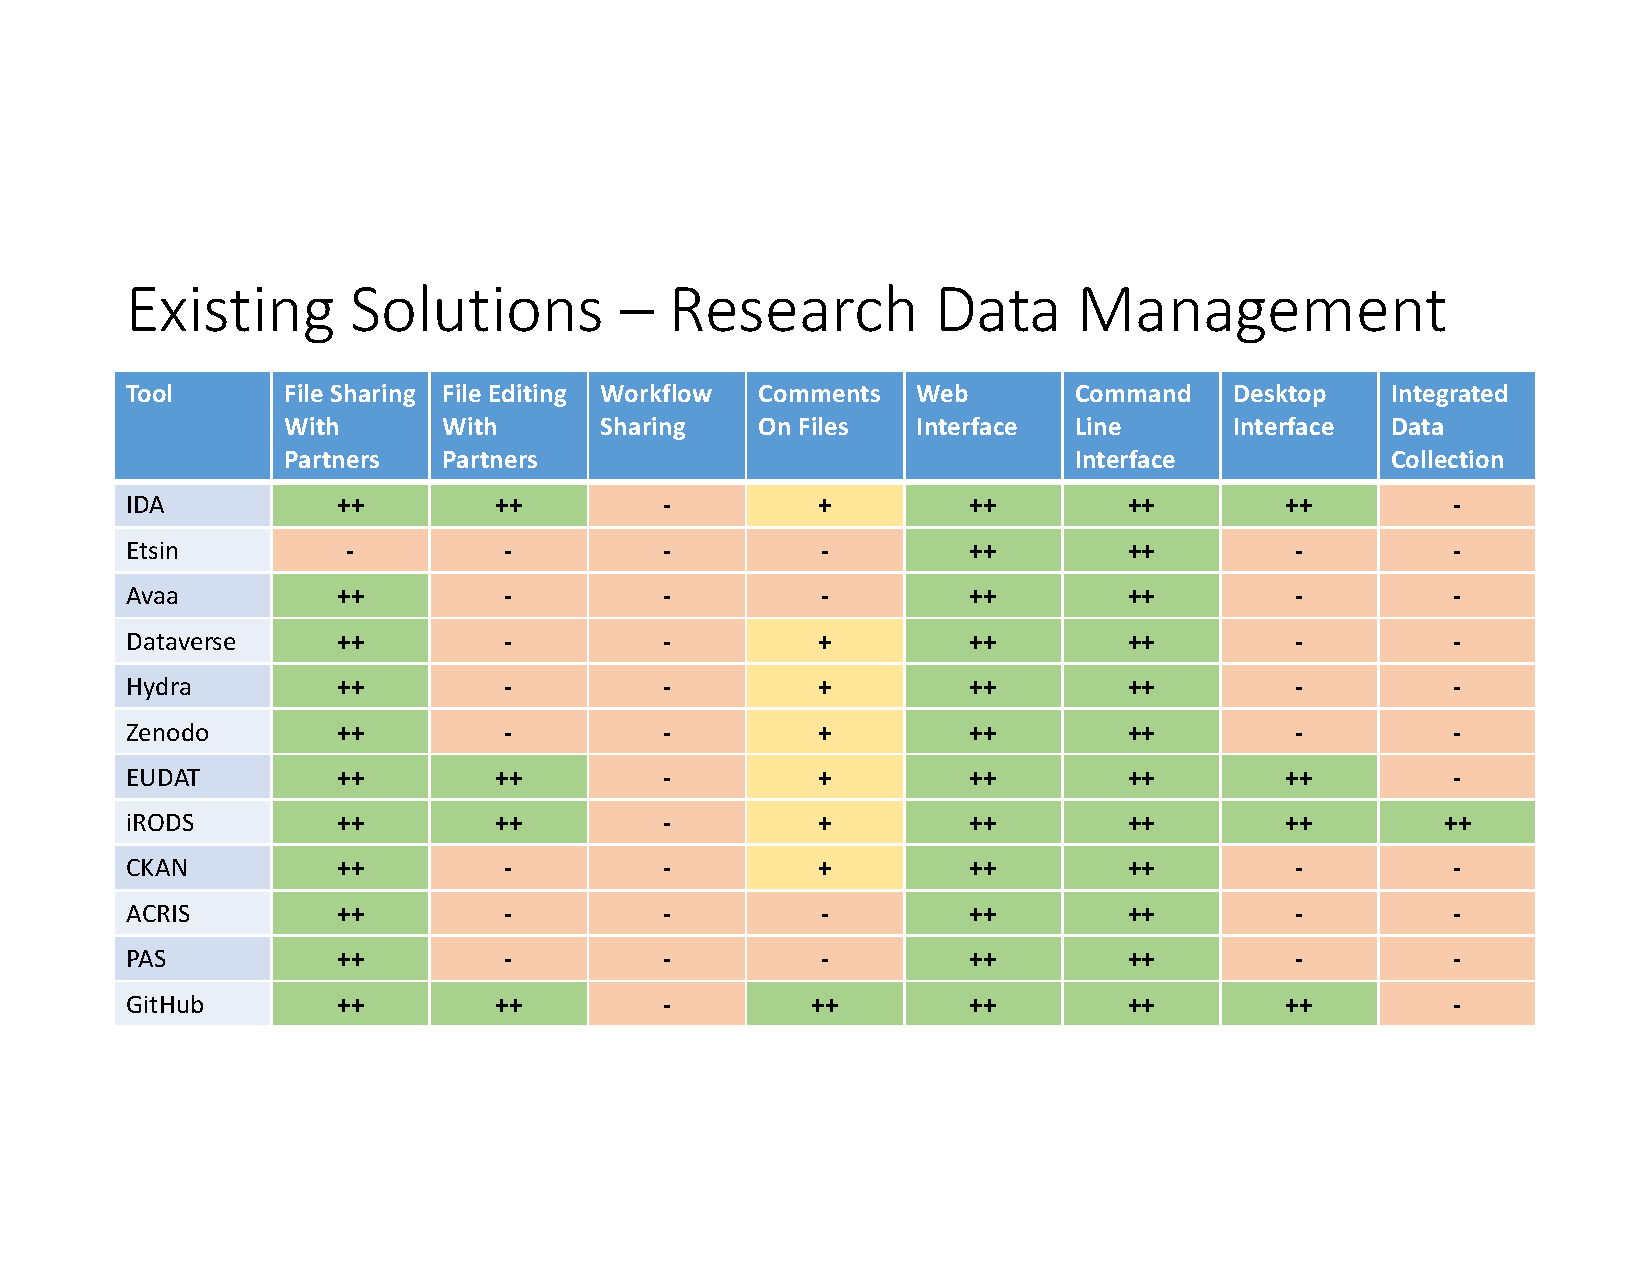
\includegraphics[width=\textwidth]{images/management}
    \end{centering}
    \caption{A placeholder for the latex table}
    \label{fig:management}
\end{sidewaysfigure}
\fi

The same tools that are suitable for research data publishing are not
necessarily right for research data management and vice versa. iRODS, IDA
and the B2Drop side offer dedicated services to share research data during
the research process and manage it in a centralized service. GitHub is a
collaborative tool for projects around programming.

This thesis has also identified many aspects of a solution that could solve the
research data management and sharing problem. These requirements are split
into functional, hardware and experiental requirements and are shown below
in Tables (TODO: put tables here). The presented requirements could be used
to design a research data management and publishing solution as well as to
validate an existing solution.

(REQUIREMENT TABLES HERE)

Technical solutions alone are not enough to make research data management
and publishing a reality. The culture about open research data has to be
changed so that it is natural and rewarding for people to publish and take
good care of their research data. This requires training, commitment from
research institutions and people to advocate for the cause.
